
\documentclass[12pt, a4paper]{report}
\usepackage{epsfig}
\usepackage{subfigure}
%\usepackage{amscd}
\usepackage{amssymb}
\usepackage{graphicx}
%\usepackage{amscd}
\usepackage{amssymb}
\usepackage{subfiles}
\usepackage{framed}
\usepackage{subfiles}
\usepackage{amsthm, amsmath}
\usepackage{amsbsy}
\usepackage{framed}
\usepackage[usenames]{color}
\usepackage{listings}
\lstset{% general command to set parameter(s)
	basicstyle=\small, % print whole listing small
	keywordstyle=\color{red}\itshape,
	% underlined bold black keywords
	commentstyle=\color{blue}, % white comments
	stringstyle=\ttfamily, % typewriter type for strings
	showstringspaces=false,
	numbers=left, numberstyle=\tiny, stepnumber=1, numbersep=5pt, %
	frame=shadowbox,
	rulesepcolor=\color{black},
	,columns=fullflexible
} %
%\usepackage[dvips]{graphicx}
\usepackage{natbib}
\bibliographystyle{chicago}
\usepackage{vmargin}
% left top textwidth textheight headheight
% headsep footheight footskip
\setmargins{3.0cm}{2.5cm}{15.5 cm}{22cm}{0.5cm}{0cm}{1cm}{1cm}
\renewcommand{\baselinestretch}{1.5}
\pagenumbering{arabic}
\theoremstyle{plain}
\newtheorem{theorem}{Theorem}[section]
\newtheorem{corollary}[theorem]{Corollary}
\newtheorem{ill}[theorem]{Example}
\newtheorem{lemma}[theorem]{Lemma}
\newtheorem{proposition}[theorem]{Proposition}
\newtheorem{conjecture}[theorem]{Conjecture}
\newtheorem{axiom}{Axiom}
\theoremstyle{definition}
\newtheorem{definition}{Definition}[section]
\newtheorem{notation}{Notation}
\theoremstyle{remark}
\newtheorem{remark}{Remark}[section]
\newtheorem{example}{Example}[section]
\renewcommand{\thenotation}{}
\renewcommand{\thetable}{\thesection.\arabic{table}}
\renewcommand{\thefigure}{\thesection.\arabic{figure}}
\title{Research notes: linear mixed effects models}
\author{ } \date{ }


\begin{document}
	\author{Kevin O'Brien}
	\title{Mixed Models for Method Comparison Studies}
	\tableofcontents
	
	%----------------------------------------------------------------------------------------%
	\newpage
	\chapter{Method Comparison Studies}

		
\section{What is a method comparison study?}
	
	% Include Somewhere: An assay is a procedure where a property is measured.
	
	The problem of compare the results of two different measurement
	techniques, or in other words, assessing the \textit{agreement} between two or more methods
	of measurement is ubiquitous in scientific research, and is
	commonly referred to as a `method comparison study'. \citet{ludbrook97} states that the purpose of comparing two measurements "of a continuous biological variable" is to uncover systematic differences, not to point to similarities". The need to compare the results of two different measurement techniques is common in medical statistics. 
	
		In particular, in medicine, new methods or devices that are cheaper, easier to use, or less invasive, are routinely developed. Agreement between a new method and either a traditional reference or gold standard must be evaluated before the new one is put into practice. Various methodologies have been proposed for this purpose in recent years.
		
	Published examples of method comparison studies can be found in disciplines	as diverse as pharmacology \citep{ludbrook97}, anaesthesia	\citep{Myles}, and cardiac imaging methods \citep{Krumm}.
	
	The approach proposed by Roy deals with the question of agreement, and indeed interchangeability, as developed by Bland and Altman's corpus of work.  In the view of Dunn, a question relevant to many practitioners is which of the two methods is more precise.
	
	
	To illustrate the characteristics of a typical method comparison
	study consider the data in Table I \citep{Grubbs73}. In each of
	twelve experimental trials, a single round of ammunition was fired
	from a 155mm gun and its velocity was measured simultaneously (and
	independently) by three chronographs devices, identified here by
	the labels `Fotobalk', `Counter' and `Terma'.
	\smallskip
		

	\begin{table}[ht]
		\begin{center}
			\begin{tabular}{rrrr}
				\hline
				Round& Fotobalk [F] & Counter [C]& Terma [T]\\
				\hline
				1 & 793.8 & 794.6 & 793.2 \\
				2 & 793.1 & 793.9 & 793.3 \\
				3 & 792.4 & 793.2 & 792.6 \\
				4 & 794.0 & 794.0 & 793.8 \\
				5 & 791.4 & 792.2 & 791.6 \\
				6 & 792.4 & 793.1 & 791.6 \\
				7 & 791.7 & 792.4 & 791.6 \\
				8 & 792.3 & 792.8 & 792.4 \\
				9 & 789.6 & 790.2 & 788.5 \\
				10 & 794.4 & 795.0 & 794.7 \\
				11 & 790.9 & 791.6 & 791.3 \\
				12 & 793.5 & 793.8 & 793.5 \\
				\hline
			\end{tabular}
			\caption{Velocity measurement from the three chronographs (Grubbs
				1973).}
		\end{center}
		\label{FCTdata}
	\end{table}
	
	An important aspect of the these data is that all three methods of
	measurement are assumed to have an attended measurement error, and
	the velocities reported in Table 1.1 can not be assumed to be
	`true values' in any absolute sense.
	
	%While lack of
	%agreement between two methods is inevitable, the question , as
	%posed by \citet{BA83}, is 'do the two methods of measurement agree
	%sufficiently closely?'
	
	A method of measurement should ideally be both accurate and
	precise. \citet{Barnhart} describes agreement as being a broader
	term that contains both of those qualities. An accurate
	measurement method will give results close to the unknown `true
	value'. The precision of a method is indicated by how tightly
	measurements obtained under identical conditions are distributed
	around their mean measurement value. A precise and accurate method
	will yield results consistently close to the true value. Of course
	a method may be accurate, but not precise, if the average of its
	measurements is close to the true value, but those measurements
	are highly dispersed. Conversely a method that is not accurate may
	be quite precise, as it consistently indicates the same level of
	inaccuracy. The tendency of a method of measurement to
	consistently give results above or below the true value is a
	source of systematic bias. The smaller the systematic bias, the
	greater the accuracy of the method.
	
	% The FDA define precision as the closeness of agreement (degree of
	% scatter) between a series of measurements obtained from multiple
	% sampling of the same homogeneous sample under prescribed
	% conditions. \citet{Barnhart} describes precision as being further
	% subdivided as either within-run, intra-batch precision or
	% repeatability (which assesses precision during a single analytical
	% run), or between-run, inter-batch precision or repeatability
	%(which measures precision over time).
	
	In the context of the agreement of two methods, there is also a
	tendency of one measurement method to consistently give results
	above or below the other method. Lack of agreement is a
	consequence of the existence of `inter-method bias'. For two
	methods to be considered in good agreement, the inter-method bias
	should be in the region of zero. A simple estimation of the
	inter-method bias can be calculated using the differences of the
	paired measurements. The data in Table 1.2 are a good example of
	possible inter-method bias; the `Fotobalk' consistently recording
	smaller velocities than the `Counter' method. Consequently one
	would conclude that there is lack of agreement between the two
	methods.
	
	The absence of inter-method bias by itself is not sufficient to
	establish whether two measurement methods agree. The two methods
	must also have equivalent levels of precision. Should one method
	yield results considerably more variable than those of the other,
	they can not be considered to be in agreement. With this in mind a
	methodology is required that allows an analyst to estimate the
	inter-method bias, and to compare the precision of both methods of
	measurement.
	\newpage
	% latex table generated in R 2.6.0 by xtable 1.5-5 package
	% Wed Aug 26 15:22:41 2009
	\begin{table}[h!]
		
		\begin{center}
			
			\begin{tabular}{rrrr}
				\hline
				Round& Fotobalk (F) & Counter (C) & F-C \\
				\hline
				1 & 793.8& 794.6 & -0.8 \\
				2 & 793.1 & 793.9 & -0.8 \\
				3 & 792.4 & 793.2 & -0.8 \\
				4 & 794.0 & 794.0 & 0.0 \\
				5 & 791.4 & 792.2 & -0.8 \\
				6 & 792.4 & 793.1 & -0.7 \\
				7 & 791.7 & 792.4 & -0.7 \\
				8 & 792.3 & 792.8 & -0.5 \\
				9 & 789.6 & 790.2 & -0.6 \\
				10 & 794.4 & 795.0 & -0.6 \\
				11 & 790.9 & 791.6 & -0.7 \\
				12 & 793.5 & 793.8 & -0.3 \\
				\hline
			\end{tabular}
			\caption{Difference between Fotobalk and Counter measurements.}
		\end{center}
	\end{table}
	

	
%=============================================================== %

	%While lack of
	%agreement between two methods is inevitable, the question , as
	%posed by \citet{BA83}, is 'do the two methods of measurement agree
	%sufficiently closely?'
	

	
	% The FDA define precision as the closeness of agreement (degree of
	% scatter) between a series of measurements obtained from multiple
	% sampling of the same homogeneous sample under prescribed
	% conditions. \citet{Barnhart} describes precision as being further
	% subdivided as either within-run, intra-batch precision or
	% repeatability (which assesses precision during a single analytical
	% run), or between-run, inter-batch precision or repeatability
	%(which measures precision over time).

	
	%----------------------------------------------------------------------------%

	\section{Agreement}
	% % - WHERE IS THIS COMING FROM?
	\citet{BA86} defined perfect agreement as the case where all of the pairs of measurement data, when plotted on a conventional scatter-plot, lie along the line of equality, where the line of equality is defined as the 45 degree line passing through the origin ,(i.e. The line $X=Y$ on the Cartesian plane). 
	
	To carry their idea a step further, we define a specific numerical measure of agreement as twice the expected squared perpendicular distance of the pair of random variables ($X_1$, $X_2$) to the line of equality or agreement in the $(X_1,X_2)$-plane, that is, $E(X_1 - X_2)/2$, where $X_1$ and $X_2$ denote the continuous measurements of rater 1 and rater 2, respectively.
	
	Obviously, other $L_p$ norms may be considered for the purpose of numerically measuring agreement and warrant future consideration. 
	
	%Note that we will use the term rater and measuring device interchangeably throughout this article.
	
	Agreement is the extent to which the measure of the variable of interest, under a constant set of experimental conditions, yields the same result on repeated trials (\textbf{Sanchez et al}). The more consistent the results, the more reliable the measuring procedure.
	




	\section{Purpose of Method Comparison Studies}
	\citet{BXC2010} provides a review of many descriptions of the purpose of Method Comparison studies, several of which are reproduced here.
	
	\begin{quote}
		``The question being answered is not always clear, but is usually epxressed as an attempt to quantify the agreement
		between two methods" \citep{BA95}.
		
		``Some lack of agreement between different methods of measurement is inevitable. What matters is the amount by which they disagree. We want to know by how much the new method is likely to differ from the old, so that it is not enough to cause problems in the mathematical interpretation we can preplace the old method by the new, or even use the two interchangeably" \citep{BA99}.
		
		
		``It often happens that the same physical and chemical property can be measured in different ways. For example, one can determine For example, one can determine sodium in serum by flame atomic emission spectroscopy or by isotope dilution mass spectroscopy. The question arises as to which method is better" (Mandel, 1991).
		
		``In areas of inter-laboratory quality control, method comparisons, assay validations and individual bio-equivalence, etc, the agreement between observations and target (reference) values is
		of interest" \citep{lin2002}.
		
		``The purpose of comparing two methods of measurement of a continuous biological variable is to uncover systematic differences, not to point to
		similarities`" \citep{ludbrook97}.
		
		``In the pharmaceutical industry, measurement methods that measure the quantity of prdocuts are regulated. The FDA (U.S. Food and Drug Administration) requires that the manufacturer show equivalency prior to approving the new or alternatice method in quality control" (Tan \& Inglewicz, 1999). 
	\end{quote}
	
	While several major commonalities are present in each definitions, there is a different emphasis for each, which will inevitably give rise to confusion. \citet{BXC2010} seems to endorse a simple phrasing of the research question that is proposed by \citet{BA83}, i.e. ``\textit{do the two methods of measurement agree sufficiently closely?}" with \citet{BXC2010} expressing the view that other considerations (for example, the ``equivalence" of two methods) to be treated as separate research questions. As such, we will revert to other research questions, such as ``equivalence of methods" later, focussing on agreement and repeatability of methods.

	


	
	
	


	

	\section{Bias as a source of Lack Of Agreement}
	Bland and Altman define bias (referred to hereafter as inter-method bias) as a \emph{a consistent tendency for one method to exceed the other} and propose estimating its value by determining the mean of the case-wise differences. 
	The variation about this mean shall be estimated by the  standard deviation of the case-wise differences. Bland and Altman remark that these estimates are based on the assumption that bias and variability are constant throughout the
	range of measures.
	%----------------------------------------------------------------------------%
	
	
	
	
	
	\section{Statement of a Model}
	\citet{BXC2010} presents a useful formulation for comparing two methods $X$ and $Y$, in their measurement of item $i$, where the unknown `true value' is $\tau_i$. Other authors, such as \citet{kinsella}, present similar formulations of the same model, as well as modified models to account for multiple measurements by each methods on each item, known as replicate measurements.
	
%	\begin{eqnarray} X_i = \tau_i + \delta_i , \phantom{spacin} \delta_i \sim \mathcal{N}(0,\sigma^2_\delta)\\ Y_i = \alpha + \beta \tau_i + \epsilon_i, \phantom{spaci}  \epsilon_i \sim \mathcal{N}(0,\sigma^2_\epsilon)\end{eqnarray}
%	
	In some types of analysis, such as the conversion problems described by \citet{lewis}, an estimate for 
	the scaling factor $\beta$ may also be sought. For the time being, we will restrict ourselves to problems where $\beta$ is assumed to be 1. 
	
	\begin{eqnarray}
		X_i = \tau_i + \delta_i , \phantom{spacin} \delta_i \sim \mathcal{N}(0,\sigma^2_\delta)\\
		Y_i = \alpha + \beta \tau_i + \epsilon_i, \phantom{spaci}  \epsilon_i \sim \mathcal{N}(0,\sigma^2_\epsilon)
	\end{eqnarray}
	
	In this formulation, $\alpha$ represents the inter-method bias, and can be estimated as $E(X-Y)$. That is to say, a simple estimate of the inter-method bias is given by the differences between pairs of measurements.  
	
	Table~\ref{FCTdata} is a good example of possible inter-method bias; the `Fotobalk' consistently recording
	smaller velocities than the `Counter' method. A cursory inspection of the table will indicate a systematic tendency for the Counter method to result in higher measurements than the Fotobalk method. % Consequently one would conclude that there is lack of agreement % between the two methods.
	

	\chapter{Improper MCS Techniques}
	
	\section{Methods of assessing agreement}

		
	Historically comparison of two methods of measurement was carried
	out by use of paired sample $t-$test, correlation coefficients or
	simple linear regression. Simple linear regression is unsuitable for method comparison studies because of the required assumption that one variable is measured without error. In comparing two methods, both methods are assume to have attendant random error.

\section{Paired sample \emph{t} test}
This method can be applied to test for statistically significant deviations in bias. This method can be potentially misused for method comparison studies. Paired t tests test only whether the mean responses are the same. Certainly, we want the means to be the same, but this is only a small part of the story. The means can be equal while the (random) differences between measurements can be huge.


\citet{Bartko} discusses the use of the well known paired sample
			$t$ test to test for inter-method bias; $H: \mu_{d}=0$. The test
			statistic is distributed a $t$ random variable with $n-1$ degrees
			of freedom and is calculated as follows,
			
			\begin{equation}
				t^{*} = \frac{\bar{d}}{ \frac{s_{d}}{\sqrt{n}}}
			\end{equation}
			
			where $\bar{d}$ and $s_{d}$ is the average of the differences of
			the $n$ observations. Only if the two methods show comparable
			precision then the paired sample student t-test is appropriate for
			assessing the magnitude of the bias.

			

			%======================================================================================= %
			
	\section{Inappropriate use of the Correlation Coefficient}
		%----------------------------------------------------------------------------%
%		\section{Pearson's Correlation Coefficient} 
% %- 			% http://www.jerrydallal.com/LHSP/compare.htm

It is well known that Pearson's correlation coefficient is a measure of the linear association between two variables, not the agreement between two variables (e.g., see Bland and Altman 1986).


This is a well known as a measure of linear association between two	variables. Nonetheless this is not necessarily the same as Agreement. This method is considered wholly inadequate to assess
		agreement because it only evaluates only the association of two sets of observations.
		
	 Use of the Pearson
	 Correlation Coefficient, although seemingly intuitive, is not
	 appropriate approach to assessing agreement of two methods.
	 Arguments against its usage have been made repeatedly in the
	 relevant literature. It is possible for two analytical methods to
	 be highly correlated, yet have a poor level of agreement.
	 	
	It is intuitive when dealing with two sets of related data, i.e
	the results of the two raters, to calculate the correlation
	coefficient (r). Bland and Altman attend to this in their $1999$
	paper.
	
	They present a data set from two sets of meters, and an
	accompanying scatterplot. An hypothesis test on the data set leads
	us to conclude that there is a relationship between both sets of
	meter measurements. The correlation coeffiecient is determined to
	be $r =0.94 $. However, this high correlation does not mean that the
	two methods agree. It is possible to determine from the
	scatterplot that the intercept is not zero, a requirement for
	stating both methods have high agreement. Essentially, should two
	methods have highly correlated results, it does not follow that
	they have high agreement.
	
It is a poor measure of agreement when the rater's measurements
are perpendicular to the line of equality[Hutson et al]. In this
context, an average difference of zero between the two raters, yet
the scatter plot displays strong negative correlation.
	

The correlation coefficient measures linear agreement--whether the measurements go up-and-down together. Certainly, we want the measures to go up-and-down together, but the correlation coefficient itself is deficient in at least three ways as a measure of agreement.

The correlation coefficient can be close to 1 (or equal to 1!) even when there is considerable bias between the two methods. For example, if one method gives measurements that are always 10 units higher than the other method, the correlation will be 1 exactly, but the measurements will always be 10 units apart.

The magnitude of the correlation coefficient is affected by the range of subjects/units studied. 

The correlation coefficient can be made smaller by measuring samples that are similar to each other and larger by measuring samples that are very different from each other. The magnitude of the correlation says nothing about the magnitude of the differences between the paired measurements which, when you get right down to it, is all that really matters.

The usual significance test involving a correlation coefficient-- whether the population value is 0--is irrelevant to the comparability problem. What is important is not merely that the correlation coefficient be different from 0. Rather, it should be close to (ideally, equal to) 1!
	




	\section*{Regression Methods}
 Regression analysis is typically misused by regressing one measurement on the other and declare them equivalent if and only if the confidence interval for the regression coefficient includes 1. Some simple mathematics shows that if the measurements are comparable, the population value of the regression coefficient will be equal to the correlation coefficient between the two methods. 
 
The population correlation coefficient may be close to 1, but is never 1 in practice. Thus, the only things that can be indicated by the presence of 1 in the confidence interval for the regression coefficient is (1) that the measurements are comparable but there weren't enough observations to distinguish between 1 and the population regression coefficient, or (2) the population regression coefficient is 1 and therefore, the measurements aren't comparable.
		
 There is a line whose slope will be 1 if the measurements are comparable. It is known as a structural equation and is the method advanced by Kelly (1985). Altman and Bland (1987) criticize it for a reason that should come as no surprise: Knowing the data are consistent with a structural equation with a slope of 1 says something about the absence of bias but *nothing* about the variability about Y = X (the difference between the measurements), which, as has already been stated, is all that really matters.

	%----------------------------------------------------------------------------%
	
	
	
	\section*{Intra-class correlation coefficient}
 
	The ICC, which takes on values between 0 and 1, is based on analysis of variance techniques. It is close to 1 when the differences between paired measurements is very small compared to the differences between subjects. Of these three procedures--t test, correlation coefficient, intra-class correlation coefficient--the ICC is best because it can be large only if there is no bias and the paired measurements are in good agreement, but it suffers from the same faults ii and iii as ordinary correlation coefficients. The magnitude of the ICC can be manipulated by the choice of samples to split and says nothing about the magnitude of the paired differences.


	%%%%%%%%%%%%%%%%%%%%%%%%%%%%%%%%%%%%%%%%%%%%%%%%%%%%%%%%%%%%%%%%%%%%%%%%%%%%%%%%%%%%%%%%%%%%%%%%%%%%%%%%%%%%%%%%%%%%%%%%
	

\chapter{Formal Testing Procedures}

\section{Formal Testing}
		The Bland-Altman plot is a simple tool for inspection of data, and	\citet{Kinsella} comments on the lack of formal testing offered by 	that methodology.
To this end, the approach proposed by \citet{BA83} is a
formal test on the Pearson correlation coefficient  of casewise
differences and means ($\rho_{AD}$). According to the authors,
this test is equivalent to a well established tests for equality
of variances, known as the `Pitman Morgan Test' \citep{Pitman,
	Morgan}.

For the Grubbs data, the correlation coefficient estimate
($r_{AD}$) is 0.2625, with a 95\% confidence interval of (-0.366,
0.726) estimated by Fishers 'r to z' transformation \citep{Cohen}.
The null hypothesis ($\rho_{AD}$ =0) would fail to be rejected.
Consequently the null hypothesis of equal variances of each method
would also fail to be rejected.

There has no been no further mention of this particular test in
the subsequent article published by Bland and Altman, although
\citet{BA99} refers to Spearmans' rank correlation coefficient.

The case-wise differences and means are calculated as $d_{i} =
x_{i}-y_{i}$ and $a_{i} = (x_{i}+y_{i})/2$  respectively. Both
$d_{i}$ and $a_{i}$ are assumed to follow a bivariate normal
distribution with $E(d_{i})= \mu_{d} = \mu_{1} - \mu_{2}$ and
$E(a_{i})= \mu_{a} = (\mu_{1} + \mu_{2})/2$. The variance matrix
$\Sigma_{(a,d)}$ is

\begin{eqnarray}
	\Sigma_{(a,d)}= \left[\begin{matrix}
		\sigma^{2}_{1}+\sigma^{2}_{2}&\frac{1}{2}(\sigma^{2}_{1}-\sigma^{2}_{2})\\
		\frac{1}{2}(\sigma^{2}_{1}-\sigma^{2}_{2})&\sigma^{2}+
		\frac{1}{4}(\sigma^{2}_{1}+\sigma^{2}_{2})
	\end{matrix} \right].
\end{eqnarray}
\section{Model for single measurement observations}
\citet{Kinsella} formulates a model for
single measurement observations for a method comparison study as a
linear mixed effects model, i.e. model that additively combine
fixed effects and random effects.
\[
Y_{ij} =\quad \mu + \beta_{j} + u_{i} + \epsilon_{ij} \qquad i = 1,\dots,n
\qquad j=1,2\]

The true value of the measurement is represented by $\mu$ while the fixed effect due to method $j$ is $\beta_{j}$.
For simplicity these terms can be combined into single terms; $\mu_{1} = \mu+ \beta_{1}$ and $\mu_{2} = \mu + \beta_{2}$. The inter-method bias is the difference of the two fixed effect terms, $\beta_{1}-\beta_{2}$. Each individual is assumed to give rise to a random error, represented by $u_{i}$. This random effects term is assumed to have mean zero and be normally distributed with variance $\sigma^2$. There is assumed to be an attendant error for each measurement on each individual, denoted $\epsilon_{ij}$. This is also assumed to have mean zero. The variance of measurement error for both methods are not assumed to be identical for both methods variance,  hence it is denoted $\sigma^2_{j}$. The set of observations ($x_{i},y_{i}$) by methods $X$ and $Y$ are assumed to follow a bivariate normal distribution with expected values $E(x_{i})= \mu_{i}$ and $E(y_{i})= \tau_{i}$ respectively. The variance covariance of the observations $\boldsymbol{\Sigma}$ is given by

\[
\boldsymbol{\Sigma} = \left[
\begin{array}{cc}
\sigma^{2} + \sigma^{2}_{1} & \sigma^{2} \\
\sigma^{2} & \sigma^{2} + \sigma^{2}_{2} \\
\end{array}
\right]
\] 
% The inter-method bias is the difference of the two fixed effect terms, $\beta_{1}-\beta_{2}$.



%%%%%%%%%%%%%%%%%%%%%%%%%%%%%%%%%%%%%%%%%%%%%%%%%%%%%%%%%%%%%%%%%%%%%%%%%%%%%%%%%%%%%%
\section{Thompson 1963: Model Formulation and Formal Testing}

\citet{Kinsella} formulates a model for un-replicated observations
for a method comparison study as a mixed model.
\begin{eqnarray}
Y_{ij} =\quad \mu_{j} + S_{i} + \epsilon_{ij} \quad i=1,2...n\quad
j=1,2\\
S \sim N(0,\sigma^{2}_{s})\qquad \epsilon_{ij} \sim
N(0,\sigma^{2}_{j}) \nonumber
\end{eqnarray}

As with all mixed models, the variance of each observation is the
sum of all the associated variance components.
\begin{eqnarray}
var(Y_{ij}) =\quad \sigma^{2}_{s} + \sigma^{2}_{j} \\
cov(Y_{i1},Y_{i2})=\quad \sigma^{2}_{s} \nonumber
\end{eqnarray}

As with all mixed models, the variance of each observation is the sum of all the associated variance components.
\begin{eqnarray}
var(Y_{ij}) =\quad \sigma^{2}_{s} + \sigma^{2}_{j} \\
cov(Y_{i1},Y_{i2})=\quad \sigma^{2}_{s} \nonumber
\end{eqnarray}

\citet{Grubbs48} offers maximum likelihood estimators, commonly
known as Grubbs estimators, for the various variance components:
\begin{eqnarray}
\hat{\sigma^{2}_{s}} \quad= \sum{\frac{(x_{i}-\bar{x})(y_{i}-\bar{y})}{n-1}}\quad=Sxy\\
\hat{\sigma^{2}_{1}} \quad= \sum{\frac{(x_{i}-\bar{x})^{2}}{n-1}} \quad=S^{2}x-Sxy \nonumber\\
\hat{\sigma^{2}_{2}} \quad=
\sum{\frac{(y_{i}-\bar{y})^{2}}{n-1}}\quad=S^{2}y-Sxy \nonumber
\nonumber
\end{eqnarray}

The standard error of these variance estimates are:
\begin{eqnarray}
var(\sigma^{2}_{1}) =\quad \frac{2\sigma^{4}_{1}}{n-1} +\quad
\frac{\sigma^2_{S}\sigma^2_{1}+\sigma^2_{S}\sigma^2_{2}+\sigma^2_{1}\sigma^2_{2}
}{n-1}\\
var(\sigma^{2}_{2}) =\quad \frac{2\sigma^{4}_{2}}{n-1} +\quad
\frac{\sigma^2_{S}\sigma^2_{1}+\sigma^2_{S}\sigma^2_{2}+\sigma^2_{1}\sigma^2_{2}
}{n-1}\nonumber
\end{eqnarray}


\citet{Kinsella} demonstrates the estimation of the variance terms and relative precisions relevant to a method comparison study, with attendant confidence intervals for both. The measurement model introduced by \citet{Grubbs48,Grubbs73} provides a formal procedure for estimating the variances $\sigma^2$, $\sigma^2_{1}$ and $\sigma^2_{2}$. \citet{Grubbs48} offers estimates, commonly known as Grubbs estimators, for the various variance components. These estimates are maximum likelihood estimates, which shall be revisited in due course.
\begin{eqnarray*}
	\hat{\sigma^{2}} = \sum{\frac{(x_{i}-\bar{x})(y_{i}-\bar{y})}{n-1}} = Sxy\\
	\hat{\sigma^{2}_{1}} = \sum{\frac{(x_{i}-\bar{x})^{2}}{n-1}} =S^{2}x - Sxy  \\
	\hat{\sigma^{2}_{2}} =
	\sum{\frac{(y_{i}-\bar{y})^{2}}{n-1}} = S^{2}y - Sxy
\end{eqnarray*}

% The standard error of these variance estimates are:
% \begin{eqnarray}
% \mbox{var}(\sigma^{2}_{1}) = \frac{2\sigma^{4}_{1}}{n-1} +
% \frac{\sigma^2_{S}\sigma^2_{1}+\sigma^2_{S}\sigma^2_{2}+\sigma^2_{1}\sigma^2_{2}
% }{n-1}\\
% \mbox{var}(\sigma^{2}_{2}) =\quad \frac{2\sigma^{4}_{2}}{n-1} +
% \frac{\sigma^2_{S}\sigma^2_{1}+\sigma^2_{S}\sigma^2_{2}+\sigma^2_{1}\sigma^2_{2}
% }{n-1}\nonumber
% \end{eqnarray}

The inter-method bias is the difference of the two fixed effect terms, $\beta_{1}-\beta_{2}$.

\citet{Kinsella} demonstrates how the Grubbs estimators for the
error variances can be calculated using the difference values,
providing a worked example on a data set.
\begin{eqnarray}
\hat{\sigma^{2}_{1}}
\quad=\sum{(y_{i1}-\bar{y{1}})(D_{i}-\bar{D})}\\
\hat{\sigma^{2}_{2}} \quad=
\sum{(y_{i2}-\bar{y_{2}})(D_{i}-\bar{D})} \nonumber
\end{eqnarray}

\citet{Thompson} presents confidence intervals for the relative
precisions of the measurement methods, $\Delta_{j}=
\sigma^2_{S}/\sigma^2_{j}$ (where $j=1,2$), as well as the
variances $\sigma^{2}_{S}, \sigma^{2}_{1}$ and $\sigma^{2}_{2}$.

\begin{eqnarray}
\Delta_{1} >\quad \frac{C_{xy}-
	t(|A|/n-2))^{\frac{1}{2}}}{C_{x}-C_{xy}+
	t(|A|/n-2))^{\frac{1}{2}}}
\end{eqnarray}
where

\begin{eqnarray}
C_{x}=\quad(n-1)S^2_{x}\nonumber\\
C_{xy}=\quad(n-1)S_{xy}\nonumber\\
C_{y}=\quad(n-1)S^2_{y}\nonumber\\
A=\quad C_{x}\times C_{y} - (C_{xy})^2 \nonumber
\end{eqnarray}

$t$ is the $100(1-\alpha/2)\%$ quantile of Student's $t$
distribution with $n-2$ degrees of freedom. $\Delta_{2}$ can be
found by changing $C_{y}$ for $C_{x}$. A lower confidence limit
can be found by calculating the square root. This inequality may
also be used for hypothesis testing.

For the interval estimates for the variance components,
\citet{Thompson} presents three relations that hold simultaneously
with probability $1-2\alpha$ where $2\alpha=0.01$ or $0.05$.

\begin{eqnarray}
|\sigma^2-C_{xy}K|\leqslant M(C_{x}C_{y})^{\frac{1}{2}}\\
|\sigma^2_{1}-(C_{x}-C_{xy})K|\leqslant M(C_{x}(C_{x}+C_{y}-2C_{xy}))^{\frac{1}{2}}\nonumber\\
|\sigma^2_{2}-(C_{y}-C_{xy})K|\leqslant
M(C_{y}(C_{x}+C_{y}-2C_{xy}))^{\frac{1}{2}}\nonumber
\end{eqnarray}











\section{Formal Models and Tests}

\citet{Thompson} defines $\Delta_j = \sigma^2 / \sigma^2_j, j=1,2$, to be a measure of the
relative precision of the measurement methods, and demonstrates how to make statistical inferences about $\Delta_{j}$.
Based on the following identities,
\begin{eqnarray*}
	C_{x}&=&(n-1)S^2_{x},\nonumber\\
	C_{xy}&=&(n-1)S_{xy},\nonumber\\
	C_{y}&=&(n-1)S^2_{y},\nonumber\\
	|A| &=& C_{x}\times C_{y} - (C_{xy})^2,\nonumber
\end{eqnarray*}
\noindent the confidence interval limits of $\Delta_{1}$ are

\begin{eqnarray}
\frac{C_{xy}-
	t(\frac{|A|}{n-2}))^{\frac{1}{2}}}{C_{x}-C_{xy}+
	t(\frac{|A|}{n-2}))^{\frac{1}{2}}} <
\Delta_{1} < \frac{C_{xy}+
	t(\frac{|A|}{n-2}))^{\frac{1}{2}}}{C_{x}-C_{xy}-
	t(\frac{|A|}{n-1}))^{\frac{1}{2}}} \nonumber
\end{eqnarray}
The value $t$ is the $100(1-\alpha/2)\%$ upper quantile of
Student's $t$ distribution with $n-2$ degrees of freedom
\citep{Kinsella}. The confidence limits for $\Delta_{2}$ are found by substituting $C_{y}$ for $C_{x}$ in (1.2).
Negative lower limits are replaced by the value $0$.
The ratio $\Delta_{2}$
can be found by interchanging $C_{y}$ and $C_{x}$. A lower
confidence limit can be found by calculating the square root. The
inequality in equation $1.10$ may also be used for hypothesis
testing.

\citet{Thompson} presents three relations that hold simultaneously
with probability $1-2\alpha$ where $2\alpha=0.01$ or $0.05$. \citet{Thompson} contains tables for $K$ and $M$.

\begin{eqnarray}
|\sigma^2-C_{xy}K|\leqslant M(C_{x}C_{y})^{\frac{1}{2}}\\
|\sigma^2_{1}-(C_{x}-C_{xy})K|\leqslant M(C_{x}(C_{x}+C_{y}-2C_{xy}))^{\frac{1}{2}}\nonumber\\
|\sigma^2_{2}-(C_{y}-C_{xy})K|\leqslant
M(C_{y}(C_{x}+C_{y}-2C_{xy}))^{\frac{1}{2}}\nonumber
\end{eqnarray}	
%For the interval estimates for the variance components,
%\citet{Thompson} presents three relations that hold simultaneously
%with probability $1-2\alpha$ where $2\alpha=0.01$ or $0.05$.

%\begin{eqnarray*}
%|\sigma^2-C_{xy}K| &\leqslant& M(C_{x}C_{y})^{\frac{1}{2}}\\
%|\sigma^2_{1}-(C_{x}-C_{xy})K|&\leqslant M(C_{x}(C_{x}+C_{y}-2C_{xy}))^{\frac{1}{2}}\nonumber\\
%|\sigma^2_{2}-(C_{y}-C_{xy})K|&\leqslant
%M(C_{y}(C_{x}+C_{y}-2C_{xy}))^{\frac{1}{2}}\nonumber
%\end{eqnarray*}

%\citet{Thompson} contains tables for $K$ and $M$.

%%%%%%%%%%%%%%%%%%%%%%%%%%%%%%%%%%%%%%%%%%%%%%%%%%%%%%%%%%%%%%%%%%%%%%%%%%%%%%%%%%%%%%


\section{Morgan Pitman}

An early contribution to formal testing in method comparison was made by both \citet{morgan} and \citet{pitman}, in separate
contributions. This test assess the equality
of population variances. Pitman's test tests for zero correlation
between the sums and products.

Correlation between differences and means is a test statistics for
the null hypothesis of equal variances given bivariate normality.


The basis of this approach is that the
distribution of the original measurements is bivariate normal.
Morgan and Pitman noted that the correlation coefficient depends
upon the difference $\sigma^{2}_{1}- \sigma^{2}_{2}$, being zero
if and only if $\sigma^{2}_{1}=\sigma^{2}_{2}$.

The classical Pitman-Morgan test is a hypothesis test for equality of the variance of two data sets; $\sigma^{2}_{1} =
\sigma^{2}_{2}$, based on the correlation value $\rho_{a,d}$ ,and is evaluated as follows;

\begin{equation}
\rho(a,d)=\quad\frac{\sigma^{2}_{1}-\sigma^{2}_{2}}{\sqrt{(\sigma^{2}_{1}+\sigma^{2}_{2})(4\sigma^{2}_{S}+\sigma^{2}_{1}+\sigma^{2}_{2})}}
\end{equation}

The test of the hypothesis that the variance of both methods are
equal is based on the correlation value $\rho_{D,A}$ which is
evaluated as follows;

\begin{equation}
\rho(D,A)=\quad\frac{\sigma^{2}_{1}-\sigma^{2}_{2}}{\sqrt{(\sigma^{2}_{1}+\sigma^{2}_{2})(4\sigma^{2}_{S}+\sigma^{2}_{1}+\sigma^{2}_{2})}}.
\end{equation}

The correlation constant takes the value zero if, and only if, the
two variances are equal. Therefore a test of the hypothesis $H:
\sigma^{2}_{1}=\sigma^{2}_{2}$ is equivalent to a test of the
hypothesis $H: \rho(D,A) = 0$. The corresponds to the well-known
$t$ test for a correlation coefficient with $n-2$ degrees of
freedom.


\citet{Bartko} describes the Morgan-Pitman test as identical to the test of the slope equal to zero in the regression of $Y_{i1}$ on $Y_{12}$, a result that can be derived using straightforward algebra.





\section{Morgan Pitman}

The test of the hypothesis that the variance of both methods are
equal is based on the correlation value $\rho_{D,A}$ which is
evaluated as follows;

\begin{equation}
	\rho(D,A)=\quad\frac{\sigma^{2}_{1}-\sigma^{2}_{2}}{\sqrt{(\sigma^{2}_{1}+\sigma^{2}_{2})(4\sigma^{2}_{S}+\sigma^{2}_{1}+\sigma^{2}_{2})}}
\end{equation}

The correlation constant takes the value zero if, and only if, the
two variances are equal. Therefore a test of the hypothesis $H:
\sigma^{2}_{1}=\sigma^{2}_{2}$ is equivalent to a test of the
hypothesis $H: \rho(D,A) = 0$. The corresponds to the well-known
$t$ test for a correlation coefficient with $n-2$ degrees of
freedom.

\citet{Bartko} describes the Morgan-Pitman test as identical to
the test of the slope equal to zero in the regression of $Y_{i1}$
on $Y_{12}$, adding that this result can be shown using
straightforward algebra.

%\subsection{Bradley & Blackwood / Pitman-Morgan Testing}
The Pitman-Morgan test for equal variances is based on the correlation of D with S. The correlation coefficient is zero if, and only if, the variances are equal. The test statistic is the familiar t-test with n-2 degree of freedom.
Bradley and Blackwood (1989) construct the conditional expectation of D given S as linear model.  They used this result to propose a test of the joint hypothesis of the mean difference and equal variances. 
If the intercept and slope estimates are zero, the two methods have the same mean and variance.
The Pitman-Morgan test is equivalent to the marginal test of the slope estimate in Bradley-Blackwood’s model.




	\section{Identifiability}
	\citet{DunnSEME} highlights an important issue regarding using models such as structural equation modelling, which is the identifiability problem. This comes as a
	result of there being too many parameters to be estimated. Therefore assumptions about some parameters, or estimators used, must be made so that others can be estimated. For example, in the literature, the variance ratio $\lambda=\frac{\sigma^{2}_{1}}{\sigma^{2}_{2}}$
	must often be assumed to be equal to $1$ \citep{linnet98}. \citet{DunnSEME} considers approaches based on two methods with single measurements on each subject as inadequate for a serious
	study on the measurement characteristics of the methods. This is because there would not be enough data to allow for a meaningful
	analysis. There is, however, a counter-argument that in many practical settings it is very difficult to get replicate observations when, for example, the measurement method requires invasive medical
	procedure.
	
	%%%%%%%%%%%%%%%%%%%%%%%%%%%%%%%%%%%%%%%%%%%%%%%%%%%%%%%%%%%%%%%%%%%%%%%%%%%%%%%
	
	
	
	%This application of the
	%Grubbs method presumes the existence of this condition, and necessitates
	%replication of observations by means external to and independent of the first
	%means. The Grubbs estimators method is based on the laws of propagation of
	%error. By making three independent simultaneous measurements on the same
	%physical material, it is possible by appropriate mathematical manipulation of
	%the sums and differences of the associated variances to obtain a valid
	%estimate of the precision of the primary means. Application of the Grubbs
	%estimators procedure to estimation of the precision of an apparatus uses
	%the results of a physical test conducted in such a way as to obtain a series
	%of sets of three independent observations.
	




	\section{Measurement Error Models}
	\citet{DunnSEME} proposes a measurement error model for use in
	method comparison studies. Consider n pairs of measurements
	$X_{i}$ and $Y_{i}$ for $i=1,2,...n$.
	\begin{equation}
		X_{i} = \tau_{i}+\delta_{i}\\
	\end{equation}
	\begin{equation}
		Y_{i} = \alpha +\beta\tau_{i}+\epsilon_{i} \nonumber
	\end{equation}
	
	In the above formulation is in the form of a linear structural
	relationship, with $\tau_{i}$ and $\beta\tau_{i}$ as the true
	values , and $\delta_{i}$ and $\epsilon_{i}$ as the corresponding
	measurement errors. In the case where the units of measurement are
	the same, then $\beta =1$.
	
	\begin{equation}
		E(X_{i}) = \tau_{i}\\
	\end{equation}
	\begin{equation}
		E(Y_{i}) = \alpha +\beta\tau_{i} \nonumber
	\end{equation}
	\begin{equation}
		E(\delta_{i}) = E(\epsilon_{i}) = 0 \nonumber
	\end{equation}
	
	The value $\alpha$ is the inter-method bias between the two
	methods.
	
	\begin{eqnarray}
		z_0 &=& d = 0 \\
		z_{n+1} &=& z_n^2+c
	\end{eqnarray}
	

	\section*{Structural Equation Modelling}
	Authors, such as a \citet{lewis}, \citet{dunnSEME} and \citet{voelkel2005center}, strongly advocate the use of \textit{Structural Equation Models} for the purposes of method comparison. Conversely \citet{BA99} also states that consider structural equation models to be inappropriate.
	


	\chapter{Regression Procedures}

	%================================================================================================= %
		\section{Regression Methods}
		Conventional regression models are estimated using the ordinary
		least squares (OLS) technique, and are referred to as `Model I
		regression' \citep{CornCoch,ludbrook97}. A key feature of Model I
		models is that the independent variable is assumed to be measured
		without error. As often pointed out in several papers
		\citep{BA83,ludbrook97}, this assumption invalidates simple linear
		regression for use in method comparison studies, as both methods
		must be assumed to be measured with error.
		
		The use of regression models that assumes the presence of error in
		both variables $X$ and $Y$ have been proposed for use instead
		\citep{CornCoch,ludbrook97}. These methodologies are collectively
		known as `Model II regression'. They differ in the method used to
		estimate the parameters of the regression.
		
		Regression estimates depend on formulation of the model. A
		formulation with one method considered as the $X$ variable will
		yield different estimates for a formulation where it is the $Y$
		variable. With Model I regression, the models fitted in both cases
		will entirely different and inconsistent. However with Model II
		regression, they will be consistent and complementary.
		
		Regression approaches are useful for a making a detailed examination of the biases across the range of measurements, allowing bias to be decomposed into fixed bias and proportional bias.
		Fixed bias describes the case where one method gives values that are consistently different
		to the other across the whole range. Proportional
		bias describes the difference in measurements getting progressively greater, or smaller, across the range of measurements. A measurement method may have either an attendant fixed bias or proportional bias, or both. \citep{ludbrook}. Determination of these biases shall be discussed in due course.
		
		

\section{Incorrect Techniques: Simple Linear Regression}


\subsubsection{Regression Analysis}
Another inappropriate approach is the regressing one set of measurements against the other. According to this methodology the measurement methods could considered equivalent if the confidence interval for
the regression coefficient included $1$. Analysts sometimes use least squares (referred to by Ludbrook as Model I) regression analysis to calibrate one method of measurement against another. In this technique, the sum of the squares of the vertical deviations of y values from the line is minimized. This approach is invalid, because both y and x values are attended by random error.


\subsubsection{The Identity Plot} This is a simple graphical approach, advocated by \citet{BA86}, that yields a cursory examination of how well the measurement methods agree. In the case of good agreement, the co-variates of the plot accord closely with the $X=Y$ line.


\subsubsection{Advantages of Regression Approaches for MCS}
\begin{itemize}
	\item These methods can be employed in conversion problems.
	\item Bland and Altman have stated that regression analysis offers insights into MCS problems.
\end{itemize}
\subsubsection{Disadvantages}
\begin{itemize}
	\item Regression methods are uninformative about the variability of the differences.
\end{itemize}

\begin{itemize}\item
	Regression methods can determine the presence of bias, and the levels of constant bias and proportional bias thereof \cite{ludbrook97,ludbrook02}.
\end{itemize}


\begin{itemize}
	\item \textbf{Constant Bias} This is a form of systematic deviations estimated as the average difference between the test
	and the reference method.
	\item \textbf{Proportional Bias} Two methods may agree on average, but they may exhibit differences over a range of measurements.
\end{itemize}

Two methods may agree on
average, but they may exhibit differences over a range of measurements.	Proportional Bias is a difference in the two measures which is proportional to the scale of the measurement. \\Using a naive estimation of bias, such as the mean of differences, it may incorrectly indicate absence of bias, by yielding a mean difference close to zero. This would be caused by positive differences in the measurements at one end of the range of measurements being canceled out by negative differences at the other end of the scale.

%------------------------------------------------------------------------%

		
		%%%%%%%%%%%%%%%%%%%%%%%%%%%%%%%%%%%%%%%%%%%%%%%%%%%%%%%%%%%%%%%%%%%%%%%%%%%%%%%%%%%%%%%%%%%%%%%%%%%%%%%%%%%%%%%%%%%%%
	\section{Blackwood-Bradley Model} 
	
	\citet{BB89} offers a formal simultaneous hypothesis test for the
	mean and variance of two paired data sets. Using simple linear
	regression of the differences of each pair against the sums, a line is fitted to the model, with estimates for intercept and slope ($\hat{\beta}_{0}$ and $\hat{\beta}_{1}$). The null hypothesis of this test is that the mean ($\mu$) and variance ($\sigma^{2}$) of both data sets are equal if the slope and
	intercept estimates are equal to zero(i.e $\sigma^{2}_{1} =
	\sigma^{2}_{2}$ and $\mu_{1}=\mu_{2}$ if and only if $\beta_{0}=
	\beta_{1}=0$ ).
	
	
	\citet{BB89} have developed a regression based procedure for
	assessing the agreement. This approach performs a simultaneous test for the equivalence of
	means and variances of the respective methods. The Bradley Blackwood test is a simultaneous test for bias and
	precision. They propose a regression approach which fits D on M,
	where D is the difference and average of a pair of results. Using simple linear
	regression of the differences of each pair against the sums, a
	line is fitted to the model, with estimates for intercept and
	slope ($\hat{\beta}_{0}$ and $\hat{\beta}_{1}$).
	%We have identified
	%this approach  to be examined to see if it can be used as a %foundation for a test perform a test on
	%means and variances individually.
	\begin{equation}
		D = (X_{1}-X_{2})
	\end{equation}
	\begin{equation}
		M = (X_{1} + X_{2}) /2
	\end{equation}
	The Bradley Blackwood Procedure fits D on M as follows:\\
	\begin{equation}
		D = \beta_{0} + \beta_{1}M
	\end{equation}
	This technique offers a formal simultaneous hypothesis test for the
	mean and variance of two paired data sets.  The null
	hypothesis of this test is that the mean ($\mu$) and variance
	($\sigma^{2}$) of both data sets are equal if the slope and
	intercept estimates are equal to zero(i.e $\sigma^{2}_{1} =
	\sigma^{2}_{2}$ and $\mu_{1}=\mu_{2}$ if and only if $\beta_{0}=
	\beta_{1}=0$ )
	
Both beta values, the intercept and slope, are derived from the respective means and
standard deviations of their respective data sets.

We determine if the respective means and variances are equal if
both beta values are simultaneously equal to zero. The Test is
conducted using an F test, calculated from the results of a
regression of D on M.

\textbf{Russell et al} have suggested this method be used in conjunction with a paired t-test , with estimates of slope and intercept.
Bradley and Blackwood have developed a regression based approach
assessing the agreement.

We have identified this approach  to be examined to see if it can
be used as a foundation for a test perform a test on means and variances individually.


	
	
	A test statistic is then calculated from the regression analysis
	of variance values \citep{BB89} and is distributed as `$F$' random
	variable. The degrees of freedom are $\nu_{1}=2$ and $\nu_{1}=n-2$
	(where $n$ is the number of pairs). The critical value is chosen
	for $\alpha\%$ significance with those same degrees of freedom.
	
	\citet{Bartko} amends this approach for use in method
	comparison studies, using the averages of the pairs, rather than
	the sums, and the corresponding case-wise differences. This approach can facilitate
	simultaneous usage of test with the Bland-Altman approach.
	Bartko's test statistic take the form:
	\[ F.test = \frac{(\Sigma d^{2})-SSReg}{2MSReg}
	\]
	
\subsection{Application to the Grubbs' Data}
For the Grubbs data, $\Sigma d^{2}=5.09 $, $SSReg = 0.60$ and
	$MSreg=0.06$ Therefore the test statistic is $37.42$, with a
	critical value of $4.10$. Hence the means and variance of the
	Fotobalk and Counter chronometers are assumed to be simultaneously
	equal.
	
	Importantly, this approach determines whether there is both
	inter-method bias and precision present, or alternatively if there
	is neither present. It has previously been demonstrated that there
	is a inter-method bias present, but as this procedure does not
	allow for separate testing, no conclusion can be drawn on the
	comparative precision of both methods.


	
	% latex table generated in R 2.6.0 by xtable 1.5-5 package
	% Mon Aug 31 15:53:51 2009
	\begin{table}[ht]
		\begin{center}
			\begin{tabular}{lrrrrr}
				\hline
				& Df & Sum Sq & Mean Sq & F value & Pr($>$F) \\
				\hline
				Averages & 1 & 0.04 & 0.04 & 0.74 & 0.4097 \\
				Residuals & 10 & 0.60 & 0.06 &  &  \\
				\hline
			\end{tabular}
			\caption{Regression ANOVA of case-wise differences and averages
				for Grubbs Data}
		\end{center}
	\end{table}
	

\section{Bradley-Blackwood Test (Kevin Hayes Talk)}
%--------------------------------------------------------------------%
% KH - UW
	
This work considers the problem of testing $\mu_1$ = $\mu_2$ and $\sigma^2_1 = \sigma^2_2$ using a random sample from a bivariate normal distribution with parameters $(\mu_1, \mu_2, \sigma^2_1, \sigma^2_2, \rho)$. 
	
The new contribution is a decomposition of the Bradley-Blackwood test statistic (\textit{Bradley and Blackwood, 1989})for the simultaneous test of {$\mu_1$ = $\mu_2$; $\sigma^2_1 = \sigma^2_2$}  as a sum of two statistics. 
	
	One is equivalent to the Pitman-Morgan (\textit{Pitman, 1939; Morgan, 1939}) test statistic 
	for $\sigma^2_1 = \sigma^2_2$ and the other one is a new alternative to the standard paired-t test of $\mu_D = \mu_1 = \mu_2 = 0$. 
	
	Surprisingly, the classic Student paired-t test makes no assumptions about the equality (or otherwise) of the 
	variance parameters. 
	
	The power functions for these tests are quite easy to derive, and show that when $\sigma^2_1 = \sigma^2_2$, 
	the paired t-test has a slight advantage over the new alternative in terms of power, but when $\sigma^2_1 \neq \sigma^2_2$, the 
	new test has substantially higher power than the paired-t test.
	
	While Bradley and Blackwood provide a test on the joint hypothesis of equal means and equal variances their regression based approach does not separate these two issues.
	
	The rejection of the joint hypothesis may be 
	due to two groups with unequal means and unequal variances; unequal means and equal variances, or equal means and unequal variances. We propose an approach for resolving this (model selection) problem in a manner controlling the magnitudes of the relevant type I error probabilities.
	
	

	\section{Deming Regression}
	
	As stated previously, the fundamental flaw of simple linear regression is that it allows for measurement error in one variable only. This causes a downward biased slope estimate.
	
	Deming regression is a regression fitting approach that assumes error in both variables. Deming regression is recommended by \citet*{CornCoch} as the
	preferred Model II regression for use in method comparison studies.
	The sum of squared distances from measured sets of values to the regression line is minimized at an angles specified by the ratio $\lambda$ of the residual variance of both variables. I
	When $\lambda$ is one, the angle is 45 degrees. In ordinary linear regression, the distances are minimized in the vertical directions \citep{linnet99}.
	In cases involving only single measurements by each method, $\lambda$ may be unknown and is therefore assumes a value of one. While this will produce biased estimates, they are less biased than ordinary linear regression.
	
	The Bland Altman Plot is uninformative about the comparative influence of proportional bias and fixed bias. Model II approaches, such as Deming regression,  can provide independent tests for
	both types of bias.
	
	For a given $\lambda$, \citet{Kummel} derived the following estimate that would later be used for the Deming regression slope
	parameter. The intercept estimate $\alpha$ is simply estimated in the same way as in conventional linear
	regression, by using the identity $\bar{Y}-\hat{\beta}\bar{X}$;
	\begin{equation}
		\hat{\beta} =\quad \frac{S_{yy} - \lambda S_{xx}+[(S_{yy} -
			\lambda S_{xx})^{2}+ 4\lambda S^{2}_{xy}]^{1/2}}{2S_{xy}}
	\end{equation}
	with $\lambda$ as the variance ratio. As stated previously $\lambda$ is often unknown, and therefore must be assumed to equal one. \citet{CarollRupert} states that Deming
	regression is acceptable only when the precision ratio ($\lambda$,in their paper as $\eta$) is correctly specified, but in practice this is often not the case, with the $\lambda$ being underestimated. Several candidate models, with varying variance ratios may be fitted, and estimates of the slope and intercept are produced. However no model selection information is available to determine the best fitting model.
	
	As with conventional regression methodologies, Deming regression calculates an estimate for both the slope and intercept for the
	fitted line, and standard errors thereof. Therefore there is sufficient information to carry out hypothesis tests on both
	estimates, that are informative about presence of fixed and proportional bias.
	
	A $95\%$ confidence interval for the intercept estimate can be used to test the intercept, and hence fixed bias, is equal to
	zero. This hypothesis is accepted if the confidence interval for the estimate contains the value $0$ in its range. Should this be,
	it can be concluded that fixed bias is not present. Conversely, if the hypothesis is rejected, then it is concluded that the
	intercept is non zero, and that fixed bias is present.
	
	Testing for proportional bias is a very similar procedure. The
	$95\%$ confidence interval for the slope estimate can be used to
	test the hypothesis that the slope is equal to $1$. This
	hypothesis is accepted if the confidence interval for the estimate
	contains the value $1$ in its range. If the hypothesis is
	rejected, then it is concluded that the slope is significant
	different from $1$ and that a proportional bias exists.
	
	For convenience, a new data set shall be introduced to demonstrate
	Deming regression. Measurements of transmitral volumetric flow
	(MF) by doppler echocardiography, and left ventricular stroke
	volume (SV) by cross sectional echocardiography in 21 patients
	with aortic valve disease are tabulated in \citet{zhang}. This
	data set features in the discussion of method comparison studies
	in \citet[p.398]{AltmanBook} .
	
	
	% latex table generated in R 2.6.0 by xtable 1.5-5 package
	% Tue Sep 01 13:31:17 2009
	\begin{table}[h!]
		\begin{center}
			\begin{tabular}{|c|c|c||c|c|c||c|c|c|}
				\hline
				Patient & MF  & SV  & Patient & MF  & SV  & Patient & MF  & SV \\
				&($cm^{3}$)&  ($cm^{3}$) & &($cm^{3}$)&  ($cm^{3}$) & &($cm^{3}$)&  ($cm^{3}$)
				\\
				\hline
				1 & 47 & 43 &  8 & 75 & 72 &  15 & 90 & 82 \\
				2 & 66 & 70 & 9 & 79 & 92 &  16 & 100 & 100 \\
				3 & 68 & 72 & 10 & 81 & 76 & 17 & 104 & 94 \\
				4 & 69 & 81 & 11 & 85 & 85 &  18 & 105 & 98 \\
				5 & 70 & 60 & 12 & 87 & 82 & 19 & 112 & 108 \\
				6 & 70 & 67 & 13 & 87 & 90 & 20 & 120 & 131 \\
				7 & 73 & 72 & 14 & 87 & 96 &  21 & 132 & 131 \\
				
				\hline
			\end{tabular}
			\caption{Transmitral volumetric flow(MF) and left ventricular
				stroke volume (SV) in 21 patients. (Zhang et al 1986)}
		\end{center}
	\end{table}
	
	
	\begin{figure}[h!]
		% Requires \usepackage{graphicx}
		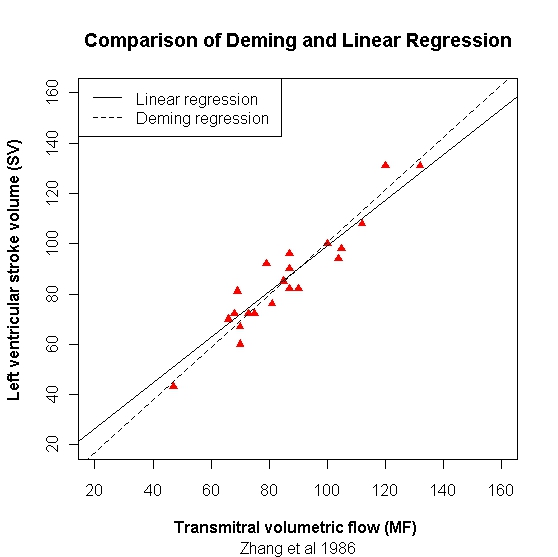
\includegraphics[width=130mm]{images/ZhangDeming.jpeg}
		\caption{Deming Regression For Zhang's Data}\label{ZhangDeming}
	\end{figure}
	
	
	\citet{CarollRupert} states that Deming's
	regression is acceptable only when the precision ratio ($\lambda$,
	in their paper as $\eta$) is correctly specified, but in practice
	this is often not the case, with the $\lambda$ being
	underestimated.
		\section{Other Types of Studies / Gold Standards}
		\citet{lewis} categorize method comparison studies into three
		different types.  The key difference between the first two is
		whether or not a `gold standard' method is used. In situations
		where one instrument or method is known to be `accurate and
		precise', it is considered as the`gold standard' \citep{lewis}. A
		method that is not considered to be a gold standard is referred to
		as an `approximate method'. In calibration studies they are
		referred to a criterion methods and test methods respectively.
		
		
		\textbf{1. Calibration problems}. The purpose is to establish a
		relationship between methods, one of which is an approximate
		method, the other a gold standard. The results of the approximate
		method can be mapped to a known probability distribution of the
		results of the gold standard \citep{lewis}. (In such studies, the
		gold standard method and corresponding approximate method are
		generally referred to a criterion method and test method
		respectively.) \citet*{BA83} make clear that their methodology is
		not intended for calibration problems.
		
		\bigskip \textbf{2. Comparison problems}. When two approximate
		methods, that use the same units of measurement, are to be
		compared. This is the case which the Bland-Altman methodology is
		specfically intended for, and therefore it is the most relevant of
		the three.
		
		\bigskip \textbf{3. Conversion problems}. When two approximate
		methods, that use different units of measurement, are to be
		compared. This situation would arise when the measurement methods
		use 'different proxies', i.e different mechanisms of measurement.
		\citet{lewis} deals specifically with this issue. In the context
		of this study, it is the least relevant of the three.
		
		\citet[p.47]{DunnSEME} cautions that`gold standards' should not be
		assumed to be error free. `It is of necessity a subjective
		decision when we come to decide that a particular method or
		instrument can be treated as if it was a gold standard'. The
		clinician gold standard , the sphygmomanometer, is used as an
		example thereof.  The sphygmomanometer `leaves considerable room
		for improvement' \citep{DunnSEME}. \citet{pizzi} similarly
		addresses the issue of glod standards, `well-established gold
		standard may itself be imprecise or even unreliable'.
		
		
		The NIST F1 Caesium fountain atomic clock is considered to be the
		gold standard when measuring time, and is the primary time and
		frequency standard for the United States. The NIST F1 is accurate
		to within one second per 60 million years \citep{NIST}.
		
		Measurements of the interior of the human body are, by definition,
		invasive medical procedures. The design of method must balance the
		need for accuracy of measurement with the well-being of the
		patient. This will inevitably lead to the measurement error as
		described by \citet{DunnSEME}. The magnetic resonance angiogram,
		used to measure internal anatomy,  is considered to the gold
		standard for measuring aortic dissection. Medical test based upon
		the angiogram is reported to have a false positive reporting rate
		of 5\% and a false negative reporting rate of 8\%. This is
		reported as sensitivity of 95\% and a specificity of 92\%
		\citep{ACR}.
		
		In literature they are, perhaps more accurately, referred to as
		`fuzzy gold standards' \citep{phelps}. Consequently when one of the methods is
		essentially a fuzzy gold standard, as opposed to a `true' gold
		standard, the comparison of the criterion and test methods should
		be consider in the context of a comparison study, as well as of a
		calibration study.



	
	
	\section{Bland Altman plots using 'Gold Standard' raters}
	According to Bland and Altman, one should use the methodology
	previous outlined, even when one of the raters is a Gold Standard.
	
	%%%%%%%%%%%%%%%%%%%%%%%%%%%%%%%%%%%%%%%%%%%%%%%%%%%%%%%%%%%%%%%%%%%%%%%%%%%%%%%%%%%%%%%%%%%%%%%%%%%%%%%%%%%%%%%%%%%%%
	%---------------------------------------------%
\chapter{Repeated Measurements and Repeatability}
	
	
	
	\section{Replicate Measurements}
	
	Thus far, the formulation for comparison of two measurement
	methods is one where one measurement by each method is taken on
	each subject. Should there be two or more measurements by each
	methods, these measurement are known as `replicate measurements'.
	\citet{BXC2008} recommends the use of replicate measurements, but
	acknowledges the additional computational complexity.
	
	\citet*{BA86} address this problem by offering two different
	approaches. The premise of the first approach is that replicate
	measurements can be treated as independent measurements. The
	second approach is based upon using the mean of the each group of
	replicates as a representative value of that group. Using either
	of these approaches will allow an analyst to estimate the inter
	method bias.
	
	%\section{Mean of Replicates Limits of Agreement}
	
	However, because of the removal of the effects of the replicate
	measurements error, this would cause the estimation of the
	standard deviation of the differences to be unduly small.
	\citet*{BA86} propose a correction for this.
	
	\citet{BXC2008} takes issue with the limits of agreement based on
	mean values of replicate measurements, in that they can only be interpreted as prediction
	limits for difference between means of repeated measurements by
	both methods, as opposed to the difference of all measurements.
	Incorrect conclusions would be caused by such a misinterpretation.
	\citet{BXC2008} demonstrates how the limits of agreement
	calculated using the mean of replicates are `much too narrow as
	prediction limits for differences between future single
	measurements'. This paper also comments that, while treating the
	replicate measurements as independent will cause a downward bias
	on the limits of agreement calculation, this method is preferable
	to the `mean of replicates' approach.
	
	
	
	%%%%%%%%%%%%%%%%%%%%%%%%%%%%%%%%%%%%%%%%%%%%%%%%%%%%%%%%%%%%%%%%%%%%%%%%%%%%%%%%%%%%%%%
	%%%%%%%%%%%%%%%%%%%%%%%%%%%%%%%%%%%%%%%%%%%%%%%%%%%%%%%%%%%%%%%%%%%%%%%%%%%%%%%%%%%%%%%
	
	
	
	
	
	\section{Repeated Measurements in LME models}
	
	In many statistical analyzes, the need to determine parameter estimates where multiple measurements are available on each of a set of variables often arises. Further to \citet{lam}, \citet{hamlett} performs an analysis of the correlation of replicate measurements, for two variables of interest, using LME models.
	
	Let $y_{Aij}$ and $y_{Bij}$ be the $j$th repeated observations of the variables of interest $A$ and $B$ taken on the $i$th subject. The number of repeated measurements for each variable may differ for each individual.
	Both variables are measured on each time points. Let $n_{i}$ be the number of observations for each variable, hence $2\times n_{i}$ observations in total.
	
	It is assumed that the pair $y_{Aij}$ and $y_{Bij}$ follow a bivariate normal distribution.
	\begin{eqnarray*}
		\left(
		\begin{array}{c}
			y_{Aij} \\
			y_{Bij} \\
		\end{array}
		\right) \sim \mathcal{N}(
		\boldsymbol{\mu}, \boldsymbol{\Sigma})\mbox{   where } \boldsymbol{\mu} = \left(
		\begin{array}{c}
			\mu_{A} \\
			\mu_{B} \\
		\end{array}
		\right)
	\end{eqnarray*}
	
	The matrix $\Sigma$ represents the variance component matrix between response variables at a given time point $j$.
	
	\[
	\boldsymbol{\Sigma} = \left( \begin{array}{cc}
	\sigma^2_{A} & \sigma_{AB} \\
	\sigma_{AB} & \sigma^2_{B}\\
	\end{array}   \right)
	\]
	
	$\sigma^2_{A}$ is the variance of variable $A$, $\sigma^2_{B}$ is the variance of variable $B$ and $\sigma_{AB}$ is the covariance of the two variable. It is assumed that $\boldsymbol{\Sigma}$ does not depend on a particular time point, and is the same over all time points.
	
	%------------------------------------------------------------------------------%
	
	
	
	\section{Definition of Replicate measurements}
	Further to \citet{BA99}, a formal definition is required of what exactly replicate measurements are
	
	\emph{By replicates we mean two or more measurements on the same
		individual taken in identical conditions. In general this requirement means that the
		measurements are taken in quick succession.}
	
	Roy accords with Bland and Altman's definition of a replicate, as being two or more measurements on the same individual under identical conditions. Roy allows the assumption that replicated measurements are equi-correlated. Roy allows unequal numbers of replicates.
	
	Replicate measurements are linked over time. However the method can be easily extended to cover situations where they are not linked over time.
	\section{Replicate measurements}
	Bland and Altman attend to the issue of repeated measures in
	$1996$.
	\\
	Repeated measurements on several subjects can be used to quantify
	measurement error, the variation between measurements of the same
	quantity on the same individual.
	\\
	Bland and Altman discuss two metrics for measurement error; the
	within-subject standard deviation ,and the correlation
	coefficient.
	
	The above plot incorporates both the conventional limits of
	agreement ( the inner pair of dashed lines), the `$t-$' limits of
	agreement ( the outer pair of dashed lines) centred around the
	inter-method bias (indicated by the full line). This plot is
	intended for expository purposes only, as the sample size is
	small.
	
	\citet{ARoy2009} accords with Bland and Altman?s definition of a replicate, as being two or more measurements on the same individual under identical conditions.
	Roy allows the assumption that replicated measurements are equi-correlated.
	Roy allows unequal numbers of replicates.
	
	
	Replicate measurements are linked over time. However the method can be easily extended to cover situations where they are not linked over time.
	
	Repeated measurements are said to be linked if a direct correspondence exists between successive measurements across measurements, i.e. pairing. Such measurements are commonly made with a time interval between them, but simultaneously for both methods. Paired measurements are exchangeable, but individual measurements are not.
	
	If the paired measurements are taken
	in a short period of time so that no real systemic changes can take place on each item, they can be considered true replicates.
	Should enough time elapse for systemic changes, linked repeated measurements can not be treated as true replicates.
	
	
	
	%%%%%%%%%%%%%%%%%%%%%%%%%%%%%%%%%%%%%%%%%%%%%%%%%%%%%%%%%%%%%%%%%%%%%%%%%%%%%%%%%%%%%%%%%%%%%%%%%%%%%%%%%%%%%%%
	
	In this model , the variances of the random effects must depend on
	$m$, since the different methods do not necessarily measure on the
	same scale, and different methods naturally must be assumed to
	have different variances. \citet{BXC2004} attends to the issue of
	comparative variances.
	
	
	
	\bigskip
	\citet{BA99} also remark that an important feature of replicate observations is that they should be independent
	of each other. This issue is addressed by \citet{BXC2010}, in terms of exchangeability and linkage. Carstenen advises that repeated measurements come in two \emph{substantially different} forms, depending on the circumstances of their measurement: exchangable and linked.
	

	%----------------------------------------------------------------------------%

	\section{Model for replicate measurements}
	
	We generalize the single measurement model for the replicate measurement case, by additionally specifying replicate values. Let $y_{mir}$ be the $r-$th replicate measurement for subject ``i" made by method ``m". Further to \citet{barnhart} fixed effect can be expressed with a single term $\alpha_{mi}$, which incorporate the true value $\mu_i$.
	
	\[ y_{mir} = \mu_{i} + \alpha_{m} + e_{mir}  \]
	
	Combining fixed effects \citep{barnhart}, we write,
	
	\[ y_{mir} = \alpha_{mi} + e_{mir}.\]
	
	The following assumptions are required
	
	\begin{itemize}
		\item $e_{mir}$ is independent of the fixed effects with mean $\mbox{E}(e_{mir}) = 0$.
		\item Further to \citet{barnhart} between-item and within-item variances $\mbox{Var}(\alpha_{mi}) = \sigma^2_{Bm}$ and $\mbox{Var}(e_{mir}) = \sigma^2_{Wm}$
		%	\item In keeping with \citet{Roy}, these variance shall be considered as part of the between-item variance covariance matrix $\boldsymbol{D}$ and the within-item variance covariance matrix  $\boldsymbol{\Sigma}$
		%	respectively, and will be denoted accordingly ( i.e. $d^2_{m}$ and $\sigma^2_{m}$).
		%	\item Additionally, the total variability of method "m", denoted $\omega^2_m$ is the sum of the within-item and between-item variabilities.
		%	
		%	\[ \omega^2_m = d^2_{m}+ \sigma^2_{m} \]
		
	\end{itemize}
	
	
	
	
		\section{Statistical Model For Replicate Measurements}
	Let $y_{Aij}$ and $y_{Bij}$ be the $j$th repeated observations of the variables of interest $A$ and $B$ taken on the $i$th subject. The number of repeated measurements for each variable may differ for each individual.
	Both variables are measured on each time points. Let $n_{i}$ be the number of observations for each variable, hence $2\times n_{i}$ observations in total.
	
	It is assumed that the pair $y_{Aij}$ and $y_{Bij}$ follow a bivariate normal distribution.
	\begin{eqnarray}
	\left(
	\begin{array}{c}
	y_{Aij} \\
	y_{Bij} \\
	\end{array}
	\right) \sim \mathcal{N}(
	\boldsymbol{\mu}, \boldsymbol{\Sigma})\mbox{   where } \boldsymbol{\mu} = \left(
	\begin{array}{c}
	\mu_{A} \\
	\mu_{B} \\
	\end{array}
	\right)
	\end{eqnarray}
	The matrix $\boldsymbol{\Sigma}$ represents the variance component matrix between response variables at a given time point $j$.
	\begin{equation}
	\boldsymbol{\Sigma} = \left( \begin{array}{cc}
	\sigma^2_{A} & \sigma_{AB} \\
	\sigma_{AB} & \sigma^2_{B}\\
	\end{array}\right)
	\end{equation}
	$\sigma^2_{A}$ is the variance of variable $A$, $\sigma^2_{B}$ is the variance of variable $B$ and $\sigma_{AB}$ is the covariance of the two variable. It is assumed that $\boldsymbol{\Sigma}$ does not depend on a particular time point, and is the same over all time points.
	
	


	\section{Linked replicates}
	
	\citet{BXC2008} proposes the addition of an random effects term to their model when the replicates are linked. This term is used to describe the `item by replicate' interaction, which is independent of the methods. This interaction is a source of variability independent of the methods. Therefore failure to account for it will result in variability being wrongly attributed to the methods.
	
	\citet{BXC2008} introduces a second data set; the oximetry study. This study done at the Royal Children�s Hospital in
	Melbourne to assess the agreement between co-oximetry and pulse oximetry in small babies.
	
	In most cases, measurements were taken by both method at three different times. In some cases there are either one or two pairs of measurements, hence the data is unbalanced. \citet{BXC2008} describes many of the children as being very sick, and with very low oxygen saturations levels. Therefore it must be assumed that a biological change can occur in interim periods, and measurements are not true replicates.
	
	\citet{BXC2008} demonstrate the necessity of accounting for linked replicated by comparing the limits of agreement from the `oximetry' data set using a model with the additional term, and one without. When the interaction is accounted for the limits of agreement are (-9.62,14.56). When the interaction is not accounted for, the limits of agreement are (-11.88,16.83). It is shown that the failure to include this additional term results in an over-estimation of the standard deviations of differences.
	
	Limits of agreement are determined using Roy's methodology, without adding any additional terms, are found to be consistent with the `interaction' model; $(-9.562, 14.504 )$. Roy's methodology assumes that replicates are linked. However, following Carstensen's example, an addition interaction term is added to the implementation of Roy's model to assess the effect, the limits of agreement estimates do not change. However there is a conspicuous difference in within-subject matrices of Roy's model and the modified model (denoted $1$ and $2$ respectively);
	\begin{equation}
	\hat{\boldsymbol{\Lambda}}_{1}= \left(\begin{array}{cc}
	16.61 &	11.67\\
	11.67 & 27.65 \end{array}\right) \qquad
	\boldsymbol{\hat{\Lambda}}_{2}= \left( \begin{array}{cc}
	7.55 & 2.60 \\
	2.60 & 18.59 \end{array} \right). 
	\end{equation}
	
	\noindent (The variance of the additional random effect in model $2$ is $3.01$.)
	
	\citet{akaike} introduces the Akaike information criterion ($AIC$), a model 
	selection tool based on the likelihood function. Given a data set, candidate models
	are ranked according to their AIC values, with the model having the lowest AIC being considered the best fit.Two candidate models can said to be equally good if there is a difference of less than $2$ in their AIC values.
	
	The Akaike information criterion (AIC) for both models are $AIC_{1} = 2304.226$ and $AIC_{2} = 2306.226$ , indicating little difference in models. The AIC values for the Carstensen `unlinked' and `linked' models are $1994.66$ and $1955.48$ respectively, indicating an improvement by adding the interaction term.
	
	The $\boldsymbol{\hat{\Lambda}}$ matrices are informative as to the difference between Carstensen's unlinked and linked models. For the oximetry data, the covariance terms (given above as 11.67 and 2.6 respectively ) are of similar magnitudes to the variance terms. Conversely for the `fat' data the covariance term ($-0.00032$) is negligible. When the interaction term is added to the model, the covariance term remains negligible. (For the `fat' data, the difference in AIC values is also approximately $2$).
	
	To conclude, Carstensen's models provided a rigorous way to determine limits of agreement, but don't provide for the computation of $\boldsymbol{\hat{D}}$ and $\boldsymbol{\hat{\Lambda}}$. Therefore the test's proposed by \citet{roy} can not be implemented. Conversely, accurate limits of agreement as determined by Carstensen's model may also be found using Roy's method. Addition of the interaction term erodes the capability of Roy's methodology to compare candidate models, and therefore shall not be adopted.
	
	Finally, to complement the blood pressure (i.e.`J vs S') method comparison from the previous section (i.e.`J vs S'), the limits of agreement are $15.62 \pm 1.96 \times 20.33 = (-24.22, 55.46)$.)
	\newpage
	
	\section{Exchangeable and Linked measurements}
	
	
	Repeated measurements are said to be exchangeable if no relationship exists between successive measurements across measurements. If the condition of exchangeability exists, a group of measurement of the same item determined by the same method can be re-arranged in any permutation without prejudice to proper analysis. There is no reason to believe that the true value of the underlying variable has changed over the course of the measurements.

	Exchangeable repeated measurements can be treated as true replicates. For the purposes of method comparison studies the following remarks can be made. The $r-$th measurement made by method $1$ has no special correspondence to the $r-$th measurement made by method $2$, and consequently any pairing of repeated measurements are as good as each other.
	
	
	%----------------------------------------------------------------------------%

	
	Replicate measurements are linked over time. However the method can be easily extended to cover situations where they are not linked over time.
	
		
	%----------------------------------------------------------------------------%
	
	

	\section{What is Repeatability}
	The quality of repeatability is the ability of a measurement method to give consistent results for a particular subject. That is to say that a measurement will agree with prior and subsequent measurements of the same subject.
	
	
	Repeatability describes the variation in measurements taken by a single method of measurement on the same item and under the same conditions. 
	A less-than-perfect test-retest reliability causes test-retest variability. Such variability can be caused by, for example, intra-individual variability and intra-observer variability. 
	A measurement may be said to be repeatable when this variation is smaller than some agreed limit.
	
	Test-retest variability is practically used, for example, in medical monitoring of conditions. In these situations, there is often a predetermined "critical difference", and for differences in monitored values that are smaller than this critical difference, the possibility of pre-test variability as a sole cause of the difference may be considered in addition to, for examples, changes in diseases or treatments.
	
	Repeatability is defined by the \textbf{IUPAC} as `\textit{the closeness of agreement between independent results obtained with the same method on identical test material, under the same conditions (same
		operator, same apparatus, same laboratory and after short intervals of time)}'  and is determined by taking multiple measurements on a series of subjects.
	
	
	
	
	
	%-----------------------------------------------------------------------------------------------------%
	\newpage
	\section{Repeatability}
	As mentioned previously, \citet{Barnhart} emphasizes the importance of repeatability as part of an overall method comparison study. The coefficient of repeatability was proposed by \citet{BA99}, and is referenced in subsequent papers, such as \citet{BXC2008}. The coefficient of repeatability is a measure of how well a
	measurement method agrees with itself over replicate measurements
	\citep{BA99}. 

		Repeatability is the ability of a measurement method to give consistent results for a particular subject, i.e. a measurement will agree with prior and subsequent measurements of the same subject. \citet{Barnhart} emphasizes the importance of repeatability as part of an overall method comparison study, a view endorsed by \citet{BXC2008}. Before there can be good agreement between two methods, a method must have good agreement with itself. If one method has poor repeatability in the sense of considerable
		variability, then agreement between two methods is bound to be
		poor \citep{ARoy2009}. 
		
		The coefficient of repeatability is a measure of how well a
		measurement method agrees with itself over replicate measurements
		\citep{BA99}. Once the the standard deviations of the differences between the two measurements (in some texts called the residual standard deviation or within-item variability) $sigma_m$ is determined, the
		computation of the coefficients of repeatability for both methods
		is straightforward. The coefficient is calculated from the (in some texts called the residual standard deviation) as  $1.96 \times \sqrt{2} \times \sigma_m$ = $2.83 \sigma_m$).
		
		\citet{Barnhart} remarks that it is important to report repeatability when assessing
		measurement, because it measures the purest form of random error
		not influenced by other factors, while further remarking `\textit{curiously replicate measurements are rarely made in method comparison studies, so that an important aspect of comparability is often overlooked}. \citet{BA99} strongly recommends the simultaneous estimation of repeatability and agreement be collecting replicated data.
		However \citet{ARoy2009} notes the lack of convenience in such calculations. 	Repeatability is defined by the \citet{IUPAC} as `\textit{the closeness of agreement between independent results obtained with the same method on identical test material, under the same conditions (same
			operator, same apparatus, same laboratory and after short intervals of time)}'  and is determined by taking multiple measurements on a series of subjects.
		
			According to the \textit{Guidelines for Evaluating and Expressing the Uncertainty of NIST Measurement Results}, the following conditions need to be fulfilled in the establishment of repeatability:
			\begin{itemize}
				\item	the same measurement procedure
				\item	the same observer
				\item	the same measuring instrument, used under the same conditions
				\item	the same location
				\item	repetition over a short period of time.
				\item  same objectives
			\end{itemize}
		
		% %	Test-retest variability is practically used, for example, in medical monitoring of conditions.
		
		A measurement is said to be repeatable when this variation is smaller than some pre-specified limit. In these situations, there is often a predetermined ``critical difference", and for differences in monitored values that are smaller than this critical difference, the possibility of pre-test variability as a sole cause of the difference may be considered in addition to, for examples, changes in diseases or treatments. \bigskip
		A measurement method can be said to have a good level of repeatability if there is consistency in repeated measurements on the same subject using that method. Conversely, a method has poor repeatability if there is considerable variation in repeated measurements.	
		
		The British Standards Institute (1979) defines a coefficient of repeatability  as \emph{the value below which the difference between two single test results may be expected to lie within a specified probability.} In the absence of other indications, the probability is 95\%.
		


	\section{Coefficient of Repeatability - Good}
	The coefficient of repeatability is a measure of how well a
	measurement method agrees with itself over replicate measurements
	\citep{BA99}. Once the within-item variability is known, the
	computation of the coefficients of repeatability for both methods
	is straightforward.
	\citet{BA99} introduces the repeatability coefficient for a method, which is defined as the upper limits of a prediction interval for the absolute difference between two measurements by the same
	method on the same item under identical circumstances \citep{BXC2008}.	
	The British standards Insitute [$1979$] define a coefficient of
	repeatability  as \emph{the value below which the difference between two single test results....may be expected to lie within a specified probability.} Unless otherwise instructed, the
	probability is assumed to be $95\%$. 
		
		$\sigma^2_{x}$ is the within-subject variance of method $x$. The repeatability coefficient is $2.77 \sigma_{x}$ (i.e. $1.96 \times \sqrt{2} \sigma_{x}$). For $95\%$ of subjects, two replicated measurement by the same method will be within this repeatability coefficient. \bigskip
		
	The Bland Altman method offers a measurement on the repeatability of the methods. The \emph{Coefficient of Repeatability} (CR) can be calculated as 1.96 (or 2) times the standard deviations of the differences between the two measurements ($d_2$ and $d_1$).
	
	
		%-------------------------------------------------------------------%

		\citet{BA99} introduces the repeatability coefficient for a method, which is defined as the upper limits of a prediction interval for the absolute difference between two measurements by the same
		method on the same item under identical circumstances \citep{BXC2008}.
		
		$\sigma^2_{x}$ is the within-subject variance of method $x$. The repeatability coefficient is $2.77 \sigma_{x}$ (i.e. $1.96 \times \sqrt{2} \sigma_{x}$). For $95\%$ of subjects, two replicated measurement by the same method will be within this repeatability coefficient.
		
		%% \section{Note 1: Coefficient of Repeatability}
		
	
	
	%	If one method has poor repeatability in the sense of considerable variability, then agreement between two methods is bound to be poor \citep{ARoy2009}.
	




	\section{Gold Standard} This is considered to be the most
	accurate measurement of a particular parameter.
		\section{Repeatability and Gold Standards}
		Currently the phrase `gold standard' describes the most accurate method of measurement available. No other criteria are set out. Further to \citet{dunnSEME}, various gold standards have a varying levels of repeatability. Dunn cites the example of the sphygmomanometer, which is prone to measurement error. Consequently it can be said that a measurement method can be the `gold standard', yet have poor repeatability. 
		
		% % % Bronze Standard
		\citet{dunnSEME} recognizes  this problem. Hence, if the most accurate method is considered to have poor repeatability, it is referred to as a ``bronze standard".  Again, no formal definition of a `bronze standard' exists.
		
		The coefficient of repeatability may provide the basis of formulation a formal definition of a `gold standard'. For example, by determining the ratio of $CR$ to the sample mean $\bar{X}$. Advisably the sample size should specified in advance. A gold standard may be defined as the method with the lowest value of $\lambda = CR /\bar{X}$ with $\lambda < 0.1\%$. Similarly, a silver standard may be defined as the method with the lowest value of $\lambda $ with $0.1\% \leq \lambda < 1\%$. Such thresholds are solely for expository purposes.
		

	\section{Importance of Repeatability in MCS}
	
		Repeatability is important in the context of method comparison because the repeatability of two methods influence the amount of agreement which is possible between those methods. If one method has poor repeatability, the agreement is bound to be poor. If both methods have poor repeatability, agreement is even worse. If one method has poor repeatability in the sense of considerable variability, then agreement between two methods is bound to be poor \citep{ARoy2009}.
		
		\citet{Barnhart} and \citet{roy} highlight the importance of reporting repeatability in method comparison, because it measures the purest random error not influenced by any external factors. Statistical procedures on within-subject variances of two methods are equivalent to tests on their respective repeatability coefficients. A formal test is introduced by \citet{roy}, which will discussed in due course.
		
	
	Barnhart emphasizes the importance of repeatability as part of an overall method comparison study. Before there can be good agreement between two methods, a method must have good agreement with itself. The coefficient of repeatability , as proposed by Bland \& Altman (1999) is an important feature of both Carstensen's and Roy's methodologies. The coefficient is calculated from the residual standard deviation (i.e. $1.96 \times \sqrt{2} \times \sigma_m$ = $2.83 \sigma_m$).
	
	
	\citet{BA99} strongly recommends the simultaneous estimation of repeatability and agreement be collecting replicated data. \citet{ARoy2009} notes the lack of convenience in such calculations.
	It is important to report repeatability when assessing measurement, because it measures the purest form of random error not influenced by other factors \citep{Barnhart}.	
	
	%% Who Said Next Line
	importance of repeatability' curiously replicate measurements are rarely made in method comparison studies, so that an important aspect of comparability is often overlooked.
	

	%--------------------------------------------------------------------%
	%\section{Bland and Altman 1999}
	As noted by Bland and Altman 1999, the repeatability of two methods of measurement can  potentially limit
	Repeatability (using Bland-Altman plot)
	The Bland-Altman plot may also be used to assess a method?s repeatability by comparing repeated measurements using one single measurement method on a sample of items.
	The plot can then also be used to check whether the variability or precision of a method is related to the size of the characteristic being measured.
	Since for the repeated measurements the same method is used, the mean difference should be zero.
	Therefore the Coefficient of Repeatability (CR) can be calculated as 1.96 (often rounded to 2) times the standard deviation of the case-wise differences.
	


	\section{Repeatability in Bland-Altman Blood Data Analysis}
	\begin{itemize}
		\item Two readings by the same method will be within $1.96
		\sqrt{2} \sigma_w $ or $2.77 \sigma_w $ for 95\% of subjects. Thisvalue is called the repeatability coefficient.
		
		\item For observer J using the sphygmomanometer $ \sigma_w = \sqrt{37.408} = 6.116$ and so the repeatability coefficient is
		$2:77 \times 6.116 = 16:95$ mmHg.
		
		\item For the machine S,$ \sigma_w = \sqrt{83.141} = 9.118$ and the repeatability coefficient is $2:77 \times 9.118 = 25.27$ mmHg.
		
		\item Thus, the repeatability of the machine is 50\% greater than that of the observer.
	\end{itemize}

		
		
		%------------------------------------------------------------------------------------------%
	\section{Carstensen Move to Chapter 2}
	\begin{itemize}
		\item The limits of agreement are not always the only issue of
		interest � the assessment of method specific repeatability and
		reproducibility are of interest in their own right.
		
		\item Repeatability can only be assessed when replicate
		measurements by each method are available.
		
		\item The repeatability coefficient for a method is defined as the
		upper limits of a prediction interval for the absolute difference
		between two measurements by the same method on the same item under
		identical circumstances.
		
		\item If the standard deviation of a measurement is $\sigma$ the
		repeatability coefficient is $2\times\sqrt{2} \sigma = 2.83\times
		\sigma \approx 2.8 \sigma$.
		
		
		\item The repeatability of measurement methods is calculated
		differently under the two models \item Under the model assuming
		exchangeable replicates (1), the repeatability is based only on
		the residual standard deviation, i.e. $2.8\sigma_m$
		
		
		\item Under the model for linked replicates (2) there are two
		possibilities depending on the circumstances.
		
		\item If the variation between replicates within item can be
		considered a part of the repeatability it will be $2.8 \sqrt{
			\omega^2 + \sigma^2_m}$.
		
		\item However, if replicates are taken under substantially
		different circumstances, the variance component $\omega^2$ may be
		considered irrelevant in the repeatability and one would therefore
		base the repeatability on the measurement errors alone, i.e. use
		$2.8 \sigma_m$.
	\end{itemize}
	
	
	
	%\section{Reproducibility}
	% 
	%It is advisable to be able to distinguish between Repeatability and a similar concept ?Reproducibility?. Reproducibility is
	
	
	
	
	
	
	
	
	
	%%========================================================================%
	%% Phase Next Section Out
	%% Where did this come from
	
	\newpage
	
	%--------------------------------------------------------------------%
	
	%--------------------------------------------------------------------%
	\section{Notes from BXC Book (chapter 9)}
	The assessment of method-specific repeatability and reproducibility is of interest in its own right.
	Repeatability and reproducibility can only be assessed when replicate measurements by each method are available.
	If replicate measurements by a method are available, it is simple to estimate the measurement error for a method, using a model with fixed effects for item, then taking the residual standard deviation as measurement error standard deviation.
	However, if replicates are linked, this may produce an estimate that biased upwards.
	The repeatability coefficient (or simply repeatability) for a method is defined as the upper limit of a
	prediction interval for the absolute difference between two measurements by the same method on the same
	item under identical circumstances (see above conditions)
	
	\[y_{mir}  = \alpha_{m} + \beta_m( \mu_i + a_{ir} + c_{mi}) + e_{mir}\]
	
	The variation between measurements under identical circumstances.
	

	
	


	%-----------------------------------------------------------------------------------------------------%
	\section{Sampling Scheme : Linked and Unlinked Replicates}
	Measurements taken in quick succession by the same observer using the same instrument on the same subject can be considered true replicates. \citet{ARoy2009} notes that some measurements may not be `true' replicates.
	
	Roy's methodology assumes the use of `true replicates'. However data may not be collected in this way. In such cases, the correlation matrix on the replicates may require a different structure, such as the autoregressive order one $AR(1)$ structure. However determining MLEs with such a structure would be computational intense, if possible at all.
	
	
	
	\emph{
		One important feature of replicate observations is that they should be independent
		of each other. In essence, this is achieved by ensuring that the observer makes each
		measurement independent of knowledge of the previous value(s). This may be difficult
		to achieve in practice.} (Check who said this
	)
	%----------------------------------------------------------------------------%
	
	
	%-----------------------------------------------------------------------------------------------------%


	
\bibliographystyle{chicago}
\bibliography{DB-txfrbib}
\end{document}
